\begin{enumerate}[label=\thesubsection.\arabic*.,ref=\thesubsection.\theenumi]
	\item Consider the lines given by
		$$L_1:x+3y-5=0$$ $$L_2:3x-ky-1=0$$ $$L_3:5x+2y-12=0.$$
		Match the Statements/Expressions in {Column I} with the Statements/Expressions in {Column II}. 
		\hfill(2008)
		\begin{tabular}{p{8cm} p{3cm}}
			Column I & Column II \\
			(A) $L_1,L_2,L_3$ are concurrent, if & (p) $k=9$ \\
			(B) One of $L_1,L_2,L_3$ is parallel to at least one of the other two, if & (q) $k=\frac{-6}{5}$ \\
			(C) $L_1,L_2,L_2$ from a triangle, if & (r) $k=\frac{5}{6}$ \\
			(D) $L_1,L_2,L_3$ do not form a triangle, if & (s) $k=5$
		\end{tabular}
\item Lines $$L_{1}: y-x=0$$ and $$L_{2}: 2x+y=0$$ intersect the line $$L_{3}: y+2=0$$ at $\vec{P}$ and $\vec{Q}$, respectively. The bisector of the acute 
angle between $L_{1}$ and $L_{2}$ intersects $L_{3}$ at $R$.\\
{STATEMENT-1 :} The ratio $PR:RQ$ equals $2\sqrt{2}:\sqrt{5}$.\\
{STATEMENT-2 :} In any triangle, bisector of an angle divides the triangle into two similar triangles.
\hfill{(2007)}
   \begin{enumerate}
   \item Statement-1 is True, Statement-2 is True; Statement-2 
is not a correct explanation for Statement-1 
   \item Statement-1 is True, Statement-2 is True; Statement-2 
is NOT a correct explanation for Statement-1 
   \item Statement-I is True, Statement-2 is False
   \item Statement-1 is False, Statement-2 is True. 
   \end{enumerate}
	\item The area enclosed within the curve $\abs{x}+\abs{y} =1$ is \rule{1cm}{0.01pt}.
    \hfill \brak{1981}
    \item $y = 10^x $ is the reflection of $y=\log x$ in the line whose equation is \rule{1cm}{0.01pt}.
    \hfill\brak{1982}
    \item The set of lines $ax+by+c=0$, where $3a+2b+4c=0$ are concurrent at the point \rule{1cm}{0.01pt}.
    \hfill\brak{1982}
    \item Given the points $\vec{A}\brak{0,4}$ and $\vec{B}\brak{0,-4}$,the equation of the locus of the point $\vec{p}\brak{x,y}$,such that 
    $\abs{AP-BP}=6$ is \rule{1cm}{0.01pt}.
    \hfill\brak{1983}
    \item If $a,b$ and $c$ are in A.P, then the straight line $ax +by +c=0$ will always pass through a fixed point whose coordinates are \rule{1cm}{0.01pt}.
    \hfill\brak{1984}
    \item The orthocentre of the triangle formed by the lines $x+y=1, 2x +3y=6$ and $4x-y+4=0$ lies in the quadrant number \rule{1cm}{0.01pt}.
    \hfill{1985}
    \item Let the algebric sum of the perpendicular distances from the points $\brak{2,0},\brak{0,2}$ and $\brak{1,1}$ to a variable straight line be zero; then the line passes through a fixed point whose coordinates are \rule{1cm}{0.01pt}.
    \hfill\brak{1991}
    \item The vertices of a triangle are $\vec{A}\brak{-1,-7}$, $\vec{B}\brak{5,1}$ and $\vec{C}\brak{1,10}$. The equation of the bisector of $\angle{ABC}$ is \rule{1cm}{0.01pt}.
    \hfill\brak{1993}
	\item For a point $\vec{P}$ in the plane, let $d_{1}(\vec{P})$ and $d_{2}(\vec{P})$ be the 
		distance of the point $\vec{P}$ from the lines $x-y=0$ and $x+y =0$ 
respectively. The area of the region $R$ consisting of all points 
		$\vec{P}$ lying in the first quadrant of the plane and satisfying
$2\leq d_{1}(\vec{P})+d_{2}(\vec{P}) \leq4$, is \rule{1cm}{0.01pt}.
		\hfill{(2014)}
	\item Let $\vec{P}=\brak{-1, 0}$, $\vec{Q}=\brak{0, 0}$ and $\vec{R}=\brak{3, 3\sqrt{3}}$ be three points. The equation of the bisector of the angle $PQR$ is \hfill{\brak{2007}}
\begin{multicols}{4}
\begin{enumerate}
\item $\frac{\sqrt{3}}{2}x+y=0$
\item $x+\sqrt{3}y=0$
\item $\sqrt{3}x+y=0$
\item $x+\frac{\sqrt{3}}{2}y=0$
\end{enumerate}
\end{multicols}
\item If one of the lines of $my^{2}+(1-m^{2})xy-mx^{2}=80$ is a bisector 
of the angle between the lines $xy=0$, then $m$ is
\hfill{(2007)}
\begin{multicols}{4}
\begin{enumerate}
\item 1
\item 2
\item -$\frac{1}{2}$
\item -2
\end{enumerate}
\end{multicols}
%
\item The perpendicular bisector of the line segment joining $\vec{P}\brak{1,4}$ and $\vec{Q}\brak{k, 3}$ has $Y$ intercept -4. Then a possible value of $k$ is \hfill{(2008)}
\begin{multicols}{4}
\begin{enumerate}
\item 1
\item 2
\item -2
\item -4
\end{enumerate}
\end{multicols} 
%
\item The shortest distance between the line $y- x =1$ and the 
	curve $x=y^{2}$ is \hfill{(2009)}
\begin{multicols}{4}
\begin{enumerate}
\item $\frac{2\sqrt{3}}{8}$
\item $\frac{3\sqrt{2}}{5}$
\item $\frac{\sqrt{3}}{4}$
\item $\frac{3\sqrt{2}}{8}$
\end{enumerate}
\end{multicols}
%
\item The lines $p\brak{p^{2}+1}x-y+q=0$ and $\brak{p^{2}+1}^{2}x+\brak{p^{2}+1}y+ 2q=0$ are perpendicular to a common line for  \hfill \brak{2009}
\begin{multicols}{2}
\begin{enumerate}
\item exactly one values of $p$
\item exactly two values of $p$ 
\item more than two values of $p$ 
\item no value of $p$ 
\end{enumerate}
\end{multicols}
%
\item Three distinct points $\vec{A}$, $\vec{B}$ and $\vec{C}$ are given in the 
2-dimensional coordinate plane such that the ratio of the 
distance of any one of them from the point $\brak{1, 0}$ to the distance from
the point $\brak{-1, 0}$ is equal to $\frac{1}{3}$. Then the circumcentre of the triangle $ABC$ is at the point: \hfill \brak{2009}
\begin{multicols}{4}
\begin{enumerate}
\item $\brak{\frac{5}{4}, 0}$
\item $\brak{\frac{5}{2}, 0}$
\item $\brak{\frac{5}{3}, 0}$
\item $\brak{0, 0}$
\end{enumerate}
\end{multicols} 

\item The line $L$ given by $\frac{x}{5}+\frac{y}{b}=1$ passes through the point $\brak{13, 32}$. The line $K$ is parallel to the line $L$ and has the equation $\frac{x}{c}+\frac{y}{3}=1$. Then the distance between $L$ and $K$ is

\hfill \brak{2010}
\begin{multicols}{4}
\begin{enumerate}
\item $\sqrt{17}$
\item $\frac{17}{\sqrt{15}}$
\item $\frac{23}{\sqrt{17}}$
\item $\frac{23}{\sqrt{15}}$
\end{enumerate}
\end{multicols} 
%
\item If the line $2x+y=k$ passes through the point which divides the line segment joining the points $\brak{1, 1}$ and $\brak{2, 4}$ in the ratio 3:2, then $k$ equals \hfill \brak{2012}
\begin{multicols}{4}
\begin{enumerate}
\item $\frac{29}{5}$
\item 5
\item 6
\item $\frac{11}{5}$
\end{enumerate}
\end{multicols} 

\item A ray of light along $x+\sqrt{3}y=\sqrt{3}$ gets reflected upon reaching the $X$ axis, the equation of the reflected ray is \hfill \brak{2013}
\begin{multicols}{2}
\begin{enumerate}
\item $y=x+\sqrt{3}$
\item $\sqrt{3}y=x-\sqrt{3}$
\item $y=\sqrt{3}x-\sqrt{3}$
\item $\sqrt{3}y=x-1$
\end{enumerate}
\end{multicols}
%
\item The $X$ coordinate of the incentre of the triangle that has the coordinates of mid points of its sides as $\brak{0, 1}$, $\brak{1, 1}$ and $\brak{1, 0}$ is
\hfill \brak{2013}
\begin{multicols}{4}
\begin{enumerate}
\item $2+\sqrt{2}$
\item $2-\sqrt{2}$
\item $1+\sqrt{2}$
\item $1-\sqrt{2}$
\end{enumerate}
\end{multicols}
%
\item Let $PS$ be the median of the triangle with vertices $\vec{P}\brak{2, 2}$, $\vec{Q}\brak{6, -1}$ and $\vec{R}\brak{7,3}$. The equation of the line passing through $\brak{1, -1}$ and parallel to $PS$ is \hfill \brak{2014}
\begin{multicols}{2}
\begin{enumerate}
\item $4x+7y+3=0$
\item $2x-9y-11=0$
\item $4x-7y-11=0$
\item $2x+9y+7=0$
\end{enumerate}
\end{multicols}

\item Let $a, b, c$ and $d$ be non-zero numbers. If the point of intersection of the lines $4ax+2ay+c=0$ and $5bx+2by+d=0$ lies in the fourth quadrant and is equidistant from the two axes then \hfill \brak{2014}
\begin{multicols}{2}
\begin{enumerate}
\item $3bc-2ad= 0$
\item $3bc+2ad=0$
\item $2bc-3ad= 0$
\item $2bc+3ad=0$ 
\end{enumerate}
\end{multicols}
%
\item The number of points, having both co-ordinates as integers, 
that lie in the interior of the triangle with vertices $\brak{0, 0}$,  $\brak{0,41}$ and $\brak{41, 0}$ is 
\hfill \brak{2015}
\begin{multicols}{4}
\begin{enumerate}
\item 820
\item 780
\item 901
\item 861
\end{enumerate}
\end{multicols}
%
\item Two sides of a rhombus are along the lines, $x-y+1=0$ and 
$7x-y-5=0$. If its diagonals intersect at $\brak{-1, -2}$, then which one of the following is a vertex of this rhombus?
%
\hfill\brak{2016}
\begin{multicols}{4}
\begin{enumerate}
\item $\brak{\frac{1}{3}, -\frac{8}{3}}$
\item $\brak{-\frac{10}{3}, -\frac{7}{3}}$
\item $\brak{-3, -9}$
\item $\brak{-3, -8}$
\end{enumerate}
\end{multicols}
%
\item A straight the through a fixed point $\brak{2, 3}$ intersects the 
	coordinate axes at distinct points $\vec{P}$ and $\vec{Q}$. If $\vec{O}$ is the origin 
and the rectangle $OPRQ$ is completed, then the locus of $R$ is
%
\hfill \brak{2018}
\begin{multicols}{2}
\begin{enumerate}
\item $2x+3y = xy$
\item $3x+2y = xy$ 
\item $3x+2y = 6xy$ 
\item $3x+2y = 6$
\end{enumerate}
\end{multicols}
%
\item Consider the set of all lines $px+qy+r=0$ such that 
$3p+2q+4r=0$. Which one of the following statements is true? 
%
\hfill \brak{2019}
\begin{enumerate}
\item The lines are concurrent at the point $\brak{\frac{3}{4}, \frac{1}{2}}$
\item Each line passes through the origin. 
\item The lines are all parallel.
\item The lines are not concurrent.
\end{enumerate}
%
\item Slope of a line passing through $\vec{P}\brak{2, 3}$ and intersecting the line $x+y=7$ at a distance of 4 units from $\vec{P}$, is
%
\hfill \brak{2019}
\begin{multicols}{4}
\begin{enumerate}
\item $\frac{1-\sqrt{5}}{1+\sqrt{5}}$
\item $\frac{1-\sqrt{7}}{1+\sqrt{7}}$
\item $\frac{\sqrt{7}-1}{\sqrt{7}+1}$
\item $\frac{\sqrt{5}-1}{\sqrt{5}+1}$
\end{enumerate}
\end{multicols}
\item The straigth lines $x+y=0$, $3x+y-4=0$, $x+3y-4=0$ form a triangle which is \hfill \brak{1983}
\begin{multicols}{2}
\begin{enumerate}   
     \item isosceles
     \item equilateral
     \item right angled
     \item none of these
\end{enumerate}
\end{multicols}
\item If $\vec{P}=\brak{1,0}$, $\vec{Q}=\brak{-1,0}$ and $\vec{R}=\brak{2,0}$ are three given points, then the locus of point $\vec{S}$ satisfing the relation $SQ^2+SR^2=2SP^2$, is 
\hfill \brak{1988}
\begin{multicols}{2}
\begin{enumerate}
    \item a straight line parallel to $X$ axis
    \item a circle passing through the origin
    \item a circle with the center at the origin 
    \item a straight line parallel to $Y$ axis 
\end{enumerate}
\end{multicols}
\item Line $L$ has intercepts $a$ and $b$ on the coordinate axes. When the axes are rotated through a given angle, keeping the origin fixed, line $L$ has intercepts $p$ and $q$. Then

\hfill \brak{1990}
\begin{multicols}{2}
\begin{enumerate}
    \item $a^2+b^2=p^2+q^2$
    \item $\frac{1}{a^2}+\frac{1}{b^2}=\frac{1}{p^2}+\frac{1}{q^2}$
    \item $a^2+p^2=b^2+q^2$
    \item $\frac{1}{a^2}+\frac{1}{p^2}=\frac{1}{b^2}+\frac{1}{q^2}$
\end{enumerate}
\end{multicols}
\item If the sum of distances of a point from two perpendicular lines in a plane is $1$, then its locus is
\hfill \brak{1992}
\begin{multicols}{2}
\begin{enumerate}
        \item square
        \item straight line
        \item circle
        \item two intersecting lines
\end{enumerate}
\end{multicols}
\item The locus of a variable point whose distance from $\brak{-2,0}$ is $\frac{2}{3}$ times its distance from the line $x=-\frac{9}{2}$ is
\hfill \brak{1994}
\begin{multicols}{2}
\begin{enumerate}
    
       \item ellipse
       \item hyperbola
       \item parabola
       \item none of these
\end{enumerate}
\end{multicols}
\item The equations to a pair of opposite sides of parallogrqam are $x^2-5x+6=0$ and $y^2-6y+5=0$, the equations to its diagnaols are 
\hfill{$\brak{1994}$}
\begin{multicols}{2}
\begin{enumerate}
      \item $x+4y=13,y=4x-7$
    \item $4x+y=13,y=4x-7$
      \item $4x+y=13,4y=x-7$
        \item $y-4x=13,y+4x=7$
\end{enumerate}
\end{multicols}
\item The orthocenter of the triangle formed by the lines $xy=0$ and $x+y=1$ is 
\hfill{$\brak{1995}$}
\begin{multicols}{4}
\begin{enumerate}
      \item $\brak{\frac{1}{2},\frac{1}{2}}$
      \item $\brak{\frac{1}{3},\frac{1}{3}}$
      \item $\brak{0,0}$
      \item $\brak{\frac{1}{4},\frac{1}{4}}$
\end{enumerate}
\end{multicols}
\item Let $PQR$ be a right angled triangle, right at $\vec{P}\brak{2,1}$. If the equation of the line $QR$ is $2x+y=3$, then the equation representing the pair of lines $PQ$ and $PR$ is
\hfill \brak{1990}
\begin{multicols}{2}
\begin{enumerate}
    \item $3x^2-3y^2+8xy+20x+10y+25=0$
    \item $3x^2-3y^2+8xy-20x-10y+25=0$
    \item $3x^2-3y^2+8xy+10x+15y+20=0$
    \item $3x^2-3y^2-8xy-10x-15y-20=0$
\end{enumerate}
\end{multicols}
\item If $x_1$,$x_2$,$x_3$ as well as $y_1$,$y_2$,$y_3$, are in G.P with the same common ratio then the points ($x_1$,$y_1$),($x_2$,$y_2$) and ($x_3$,$y_3$).
\hfill{$\brak{1999}$}
\begin{multicols}{2}
\begin{enumerate}
        \item lie on a straight line
        \item lie on ellipse
        \item lie on circle
        \item are vertices of a triangle 
\end{enumerate}
\end{multicols}
\item Let $PS$ be the median of the triangle with vertices $\vec{P}\brak{2,2}$, $\vec{Q}\brak{6,-1}$ and $\vec{R}\brak{7,3}$. The equation of the line passing through $\brak{1,-1}$ and parallel to $PS$ is 
\hfill{$\brak{2000}$}
\begin{multicols}{2}
\begin{enumerate}
      \item $2x-9y-7=0$  
      \item $2x-9y-11=0$
      \item $2x+9y-11=0$
      \item $2x+9y+7=0$
\end{enumerate}
\end{multicols}
\item The incentre of the triangle with vertices $\brak{1,\sqrt{3}}$, $\brak{0,0}$ and $\brak{2,0}$ is 
\hfill{$\brak{2000}$}
\begin{multicols}{4}
\begin{enumerate}
     \item $\brak{1,\frac{\sqrt{3}}{2}}$
     \item $\brak{\frac{2}{3},\frac{1}{\sqrt{3}}}$
     \item $\brak{\frac{2}{3},\frac{\sqrt{3}}{2}}$
     \item $\brak{1,\frac{1}{\sqrt{3}}}$
\end{enumerate}
\end{multicols}
\item the number of integer values of $m$, for which the x-coordinate of the point of intersection of the lines $3x+4y=9$ and $y=mx+1$ is also an integer, is 
\hfill{$\brak{2001}$}
\begin{multicols}{4}
\begin{enumerate}
    \item $2$
    \item $0$
     \item $4$
     \item $1$
\end{enumerate}
\end{multicols}
\item Area of the parallelogram formed by the lines $y=mx$, $y=mx+1$, $y=nx$ and $y=nx+1$ equals
\hfill{$\brak{2001}$}
\begin{multicols}{4}
\begin{enumerate}
    
     \item $\frac{\abs{m+n}}{\brak{m-n}^2}$
     \item $\frac{2}{\abs{m+n}}$
     \item $\frac{1}{\abs{m+n}}$
     \item $\frac{1}{\abs{m-n}}$
    
\end{enumerate}
\end{multicols}
\item Let $0 < \alpha < \frac{\pi}{2}$ be a fixed angle. If
$\vec{P}=\brak{\cos\theta,\sin\theta}$ and $\vec{Q}=\brak{\cos\brak{\alpha-\theta}, \sin\brak{\alpha-\theta}}$, then $\vec{Q}$ is obtained from $\vec{P}$ by
\hfill{$\brak{2002}$}
\begin{enumerate}
    \item clockwise rotation around origin through an angle $\alpha$
    \item anticlockwise rotation around the orgin through an angle $\alpha$
    \item reflection in the line through origin with the slope $\tan\alpha$
    \item reflection in the line through origin with slope $\tan\brak{\frac{\alpha}{2}}$
\end{enumerate}
\item Let $\vec{P}=\brak{-1,0}$,$\vec{Q}=\brak{0,0}$ and $\vec{R}=\brak{3,\sqrt{3}}$ be three points. Then the equation of the bisector of the angle $PQR$ is 
\hfill{$\brak{2002}$}
\begin{multicols}{2}
\begin{enumerate}
    
        \item $\frac{\sqrt{3}}{2}x+y=0$
        \item $x+\sqrt{3}y=0$
        \item $\sqrt{3}+y=0$
        \item $x+\frac{\sqrt{3}}{2}y=0$
    
\end{enumerate}
\end{multicols}
\item A straigth line through the origin $\vec{O}$ meets the parallel lines $4x+2y=9$ and $2x+y+6=0$ at points $\vec{P}$ and $\vec{Q}$ respectively. Then the point $\vec{O}$ divides the segment $PQ$ in the ratio 
\hfill{$\brak{2002}$}
\begin{multicols}{4}
\begin{enumerate}

     \item $\ratio{1}{2}$
     \item $\ratio{3}{4}$
     \item $\ratio{2}{1}$
     \item $\ratio{4}{3}$

\end{enumerate}
\end{multicols}
\item                    	
	\begin{enumerate}
             \item  Two vertices of a triangle are \brak{5,-1} and \brak{2,-3}. If the orthocentre of the triangle is the origin, find the coordinates of the third point.
	     \item  Find the equation of the line which bisects the obtuse angle between  the lines $x-2y+4=0$ and $4x-3y+2=0$.
         \end{enumerate}\hfill{(1979)}

\item A stright line $L$ is perpendicular to the line $5x-y+1$. The area of the triangle formed by $L$ and the coordinate axes is 5. Find the equation of the line $L$.\hfill{(1980)}

\item The ends $\vec{A}$, $\vec{B}$ of a straight line segment of constant lenght $c$ slide upon the fixed rectangular axes $ OX, OY$ respectively. If the rectangle $OAPB$ be completed, then show that the locus of the foot of perpendicular drawn from $\vec{P}$ to $AB$ is 
 \begin{align*}  x^\frac{2}{3} + y^\frac{2}{3} = c^\frac{2}{3} \end{align*}
  \item The vertices of a triangle are $\sbrak{ at_1t_2,a\brak{t_1+t_2}}, \sbrak{ at_2t_3,a\brak{t_2+t_3}},\sbrak{at_3t_1,a\brak{t_3+t_1}}$. Find the orthocentre of the triangle. \hfill{(1983)}
	 % 
  \item The coordinates of $\vec{A},\vec{B},\vec{C}$ are $ \brak{6,3}, \brak{3,5}, \brak{4,2} $ respectively, and $\vec{P}$ is any point $(x,y)$.
Show that the ratio of the area of $\triangle$s $PBC$  and $ABC$ is $\abs{\frac{x+y-2}{7}}$ \hfill{(1983)} 
%
\item Two equal sides of an isosceles triangle are given by the equations $7x-y+3=0$ and $x+y-3=0$ and its third side passes through the point $\brak{1,-10}$. Determine the equation of the third side.  \hfill{(1985)}
%
\item One of the diameters of the circle circumscribing the rectangle $ABCD$ is $4y=x+ 7$. If $\vec{A}$ and $\vec{B}$ are the points $\brak{-3,4}$ and $\brak{5,4}$ respectively, the find the area of rectangle.  \hfill{(1985)}
%
\item Two sides of a rhombus $ABCD$ are parallel to the lines $y=x+2$ and $y=7x+3$. If the diagonals of the rhombus intersect at the point $\brak{1,2}$ and the vertex $\vec{A}$ is on the $Y$ axis, find the possible co-ordinates of $\vec{A}$.     \hfill{(1985)} 
%
\item Lines $ L_1 \equiv ax+by+c =0 $ and $ L_2 \equiv lx+my+n =0 $ intersect at the point $\vec{P}$ and make an angle $\theta$ with each other. Find the equation of a line $L$ different from $L_2$ which passes through $\vec{P}$ and makes same angle $\theta$ with $L_1$. \hfill{(1988)}
%
\item Let $ABC$ be the triangle $AB=AC$. If $\vec{D}$ is the midpoint of $ BC, \vec{E}$ is the foot of the perpendicular drawn from $\vec{D}$ to $AC$ and $\vec{F}$ the mid-point of $DE$, prove that $AF$ is perpendicular to $BE$. \hfill{(1989)}
%
\item Straight lines $3x + 4y =5$ and $ 4x-3y= 15$ intersect at the point $\vec{A}$. Points $\vec{B}$ and $\vec{C}$ are chosen on these two lines such that $AB=AC$. Determine the possible equations of the line $BC$ passing through the point $\brak{1,2}$. \hfill{(1990)}
%
\item A line cuts the $X$ axis at $\vec{A}(7,0)$ and the $Y$ axis at $\vec{B}(0,-5)$. A variable line $PQ$ is drawn perpendicular to $AB$ cutting the $X$ axis in $\vec{P}$ and the $Y$ axis in $\vec{Q}$. If $AQ$ and $BP$ intersect at $\vec{R}$, find the locus of $\vec{R}$.  \hfill{(1990)}
%
\item Find the equation of the line passing through the point $\brak{2,3}$ and making intercept of length 2 units between the lines $ y + 2x = 3 $ and $ y + 2x = 5  $.     \hfill{(1991)}
  \begin{center}
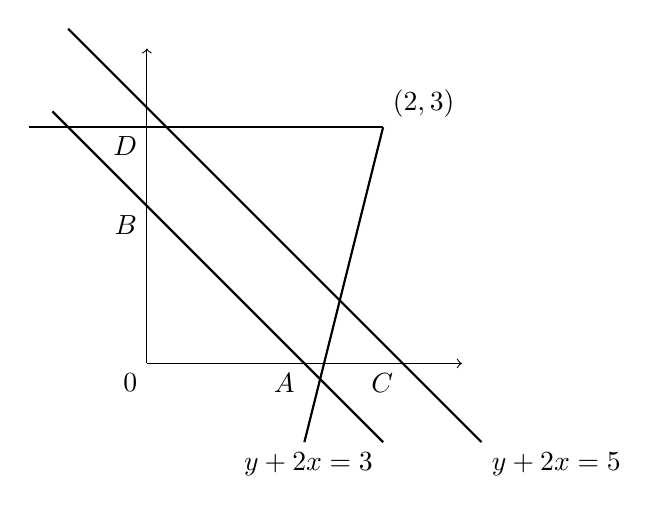
\begin{tikzpicture}
   
\draw[->] (0,0) -- (4,0) node[right] {};
\draw[->] (0,0) -- (0,4) node[above] {};


\draw[thick] (-1,4.25) -- (4.25,-1) node[below right] {$y + 2x = 5$};
\draw[thick] (-1.2,3.2) -- (3,-1) node[below left] {$y + 2x = 3$};


\filldraw[black] (0,0)  node[below left] {$0$};
\filldraw[black] (2,0)  node[below left] {$A$};
\filldraw[black] (3.25,0)  node[below left] {$C$};
\filldraw[black] (3,3)  node[above right] {$(2,3)$};


\draw[thick] (-1.5,3) -- (3,3) node[midway, right] {};

\draw[thick] (2,-1) -- (3,3) node[midway, right] {};


\node[below left ] at (0,2) {$B$};
\node[below left ] at (-0,3) {$D$};
\end{tikzpicture}
\end{center}
%	
\item Show that all chords of  the curve $ 3x^2-y^2-2x+4y=0,$ which subtend a right angle at the origin, pass through a fixed point. Find the coordinates of the point.     \hfill{(1991)}
%
\item Determine all values of $\alpha$ for which the point ($\alpha , \alpha^2$) lies inside the triangle formed by the lines.  \hfill{(1992)}
	\begin{align*}  2x+3y-1&=0\\ 
	x+2y-3&=0  \\ 5x-6y-1&=0   \end{align*}
%
\item A line through $\vec{A} \brak{5, 4}$ meets the lines $x+3y+2=0$, $2x+y+4=0$ and $x-y-5=0$ at the points $\vec{B}$, $\vec{C}$ and $\vec{D}$ respectively. If $\brak{\frac{15}{AB}}^{2}+\brak{\frac{10}{AC}}^{2}-\brak{\frac{6}{AD}}^{2}$, find the equation of the line.
	\hfill{(1993)}
%
\item A rectangle $PQRS$ has its side $PQ$ parallel to the line $y=mx$ 
	and vertices $\vec{P}$, $\vec{Q}$ and $\vec{S}$ on the lines $y=a$, $x=b$ and $x=-b$, 
		respectively. Find the locus of the vertex $\vec{R}$.
		\hfill{(1996)}
%
\item For points $\vec{P}=\brak{x_{1}, y_{1}}$ and $\vec{Q}=\brak{x_{2}, y_{2}}$ of the co-ordinate plane, a new distance $d\brak{\vec{P}, \vec{Q}}$ is defined by $d\brak{\vec{P}, \vec{Q}}=\abs{x_{1}-x_{2}}+\abs{y_{1}-y_{2}}$. Let $\vec{O}=\brak{0, 0}$ and $\vec{A}=\brak{3, 2}$. Prove that the set of points in the first quadrant which are equidistant (with respect to the new distance) from $\vec{O}$ and $\vec{A}$ consists of the union of a line segment of finite length and an infinite ray. Sketch this net in a labelled diagram.
	\hfill{(2000)}
%
\item Let $ABC$ and $PQR$ be any two triangles in the same plane.
	Assume that the perpendiculars from the points $\vec{A, B, C}$ to 
		the sides $QR, RP, PQ$ respectively are concurrent. Using vector methods or otherwise, prove that the perpendiculars from $\vec{P, Q, R}$ to $BC, CA, AB$ respectively are also concurrent. 
	\hfill{(2000)}
%
\item Let $a, b, c$ be real numbers with $a^{2}+b^{2}+c^{2}=1$. Show that the equation 
	\begin{align*}
		\mydet{
ax-by-c     &bx+ay       &cx+a      \\
bx+ay       &-ax+by-c   &cy+b       \\
cx+a         &cy+b         &-ax-by+c } =0
	\end{align*}
represents a straight line.
\hfill{(2001)}
%
\item A straight line $L$ through the origin meets the lines $x+y=1$ and $x+y=3$ at $\vec{P}$ and $\vec{Q}$ respectively. Through $\vec{P}$ and $\vec{Q}$ two 
	straight lines $L_{1}$, and $L_{2}$ are drawn, parallel to $2x-y=5$ and $3x+y=5$ respectively. Lines $L_{1}$ and $L_{2}$ intersect at $\vec{R}$. Show 
		that the locus of $\vec{R}$ as $L$ varies, is a straight line. 
\hfill{(2002)}
%
\item A straight line $L$ with negative slope passes through the 
point \brak{8, 2} and cuts the positive coordinate axes at points 
		$\vec{P}$ and $\vec{Q}$. Find the absolute minimum value of $OP + OQ$, as $L$ 
varies, where $\vec{O}$ is the origin.
%
\hfill{(2002)}
%
\item The area of the triangle formed by the intersection of a line 
	parallel to $X$ axis and passing through $\vec{P}\brak{h, k}$ with the lines 
$y=x$ and $x+y=2$ is $4h^{2}$. Find the locus of the point $\vec{P}$.
%
\hfill{(2005)}
    \item The straight line $5x+4y=0$ passes through the point of intersection of the straight lines $x+2y-10=0$ and $2x+y+5=0$.
    \hfill \brak{1983}
    \item The lines $2x+3y+19=0$ and $9x+6y-17=0$ cut the coordinates axes in concylic points.
    \hfill \brak{1988}
    \item If $$ 
	    \myvec{
a & a^2 & 1+a^3\\
b & b^2 & 1+b^3\\
c & c^2 & 1+c^3
}
=0$$
and the vectors $\vec{A}$=(1,a,$a^2$), $\vec{B}$=(1,b,$b^2$), $\vec{C}$=(1,c,$c^2$) are co-planar, then the product $abc$=\rule{1cm}{0.01pt}.
\hfill {(1985)}
\item If the vectors $a\hat{i}+\hat{j}+\hat{k}$,$\hat{i}+b\hat{j}+\hat{k}$ and $\hat{i}+\hat{j}+c\hat{k}$ $(a\neq b\neq c\neq 1)$ are co-planar, then the value of the $\frac{1}{(1-a)}$+$\frac{1}{(1-b)}$+$\frac{1}{(1-c)}$=\rule{1cm}{0.01pt}.
\hfill{(1987)}
\item A non-zero vector $\vec{a}$ is parallel to the line of intersection of the plane determined by the vectors $\hat{i}$, $\hat{i}+\hat{j}$ and the plane determined by the vectors $\hat{i}-\hat{j}$, $\hat{i}+\hat{k}$. The angle between $\vec{a}$ and the vector $\hat{i}-2\hat{j}+2\hat{k}$ is \rule{1cm}{0.01pt}.
\hfill{(1996)}
\item %23
	Three lines $$L_1:\vec{r}=\lambda\hat{i}, \lambda\in R$$ 
		$$L_2:\vec{r}=\hat{k}+\mu\hat{j}, \mu\in R$$ and
		$$L_3:\vec{r}=\hat{i}+\hat{j}+\nu\hat{k}, \nu\in R$$
		are given. For which point\brak{s} $\vec{Q}$ on $L_2$ can we find a point $\vec{P}$ on $L_1$ and a point $\vec{R}$ on $L_3$ so that $\vec{P},\vec{Q}$ and $\vec{R}$ are collinear? \hfill{\brak{2019}}
\begin{multicols}{4}
  \begin{enumerate}
	  \item $\hat{k}-\frac{1}{2}\hat{j}$
	  \item $\hat{k}$
	  \item $\hat{k}+\hat{j}$
	  \item $\hat{k}+\frac{1}{2}\hat{j}$
   \end{enumerate}
\end{multicols}
	\item If the straight lines $\frac{x-1}{2}=\frac{y+1}{k}=\frac{z}{2}$ and $\frac{x+1}{5}=\frac{y+1}{2}=\frac{z}{k}$ are coplanar, then the plane(s) containing these two lines is(are) \hfill{(2012)}
\begin{multicols}{4}
		\begin{enumerate}
			\item $y+2z=-1$
			\item $y+z=-1$
			\item $y-z=-1$
			\item $y-2z=-1$
		\end{enumerate}
\end{multicols}
%12
	\item A line $L$ passing through the origin is perpendicular to the lines
		\begin{align*}
			l_1 : \brak{3+t}\hat{i}+\brak{1+2t}\hat{j}+\brak{4+2t}\hat{k},\quad -\infty<t<\infty \\
			l_2 : \brak{3+2s}\hat{i}+\brak{3+2s}\hat{j}+\brak{2+s}\hat{k}, \quad -\infty<s<\infty 
		\end{align*}
		Then, the coordinate(s) of the point(s) on $l_2$ at a distance of $\sqrt{17}$ from the point of intersection of $L$ and $l_1$ is (are) \hfill{(2013)}
\begin{multicols}{4}
		\begin{enumerate}
			\item $\brak{\frac{7}{3},\frac{7}{3},\frac{5}{3}}$
			\item $\brak{-1,-1,0}$
			\item $\brak{1,1,1}$
			\item $\brak{\frac{7}{9},\frac{7}{9},\frac{8}{9}}$
		\end{enumerate}
\end{multicols}
%13
	\item Two lines $$L_1: x=5,\frac{y}{3-\alpha}=\frac{z}{-2}$$ and $$L_2: x=\alpha,\frac{y}{-1}=\frac{z}{2-\alpha}$$ are coplanar. Then $\alpha$ can take value(s) \hfill{(2013)}
\begin{multicols}{4}
		\begin{enumerate}
			\item 1
			\item 2 
			\item 3
			\item 4
		\end{enumerate}
\end{multicols}
	\item From a point $\vec{P}\brak{\lambda,\lambda,\lambda}$, perpendiculars $PQ$ and $PR$ are drawn respectively on the lines $y=x,z=1$ and $y=-x,z=-1$. If $\angle QPR$ is a right angle, then
		the possible value(s) of $\lambda$ is/(are) \hfill{(2014)}
\begin{multicols}{4}
		\begin{enumerate}
			\item $\sqrt{2}$
			\item 1 
			\item -1 
			\item -$\sqrt{2}$
		\end{enumerate}
\end{multicols}
%16
	\item In $R^3$, consider the planes $P_1:y=0$ and $P_2:x+z-1$. Let $P_3$ be the plane different from $P_1$ and $P_2$ which passes through the intersection of $P_1$ and $P_2$. If the distance of the
		point \brak{0,1,0} from $P_3$ is 1 and the distance of point $\brak{\alpha,\beta,\gamma}$ from $P_3$ is 2,  then which of the following relations is (are) true \hfill{(2015)}
\begin{multicols}{2}
		\begin{enumerate}
			\item $2\alpha+\beta+2\gamma+2=0$
			\item $2\alpha-\beta+2\gamma+4=0$
			\item $2\alpha+\beta+2\gamma-10=0$
			\item $2\alpha-\beta+2\gamma-8=0$
		\end{enumerate}
\end{multicols}
%17
	\item In $R^3$, let $L$ be a straight line passing through the origin. Suppose that all the points on $L$ are at a constant distance from two planes $P_1:x+2y-z+1=0$ and $P_2:2x-y+z-1=0$. Let $M$ be the
		locus of the feet of the perpendicular drawn from the points on $L$ to the plane $P_1$. Which of the following points lie(s) on M? \hfill{(2015)}
\begin{multicols}{2}
		\begin{enumerate}
			\item $\brak{0,-\frac{5}{6},-\frac{2}{3}}$
			\item $\brak{-\frac{1}{6},-\frac{1}{3},\frac{1}{6}}$
			\item $\brak{-\frac{5}{6},0,\frac{2}{3}}$
			\item $\brak{-\frac{1}{3},0,\frac{2}{3}}$
		\end{enumerate}
\end{multicols}
	\item Consider a pyramid $OPQRS$ located in the first octant $(x\geq 0,y\geq 0,z\geq 0)$ with $\vec{O}$ as origin, and $OP$ and $OR$ along the $X$ axis and the $Y$ axis respectively. The base $OPQR$ of the pyramid is
		a square with $OP=3$. The point $\vec{S}$ is directly above the mid-point $\vec{T}$ of diagonal $OQ$ such that $TS$=3. Then \hfill{(2016)}
		\begin{enumerate}
			\item the acute angle between $OQ$ and $OS$ is $\frac{\pi}{3}$
			\item the equation of the plane containg the triangle $OQS$ is $x-y=0$
			\item the length of the perpendicular from $\vec{P}$ to the plane containing the triangle $OQS$ is $\frac{3}{\sqrt{2}}$
			\item the perpendicular distance from $\vec{O}$ to the straight line containing $RS$ is $\sqrt{\frac{15}{2}}$
		\end{enumerate}
	\item Let $P_1:2x+y-z=3$ and $P_2:x+2y+z=2$ be two planes. Then, which of the following statement(s) is(are) TRUE? \hfill{(2018)}
		\begin{enumerate}
			\item The line of intersection of $P_1$ and $P_2$ has direction ratios 1,2,-1
			\item The line $\frac{3x-4}{9}=\frac{1-3y}{9}=\frac{z}{3}$ is perpendicular to the line of intersection of $P_1$ and $P_2$
			\item The acute angle between $P_1$ and $P_2$ is $60\degree$.
			\item If $P_3$ is the plane passing through the point \brak{4,2,-2} and perpendicular to the line of intersection of $P_1$ and $P_2$, then the distance of the point \brak{2,1,1}
				from the plane $P_3$ is $\frac{2}{\sqrt{3}}$
		\end{enumerate}
%22
	\item Let $L_1$ and $L_2$ denote the lines\\ $\vec{r}=\hat{i}+\lambda\brak{-\hat{i}+2\hat{j}+2\hat{k}}, \lambda \in R$ and \\
		$\vec{r}=\mu \brak{2\hat{i}-\hat{j}+2\hat{k}}, \mu \in R$\\ respectively. If $L_3$ is a line which is perpendicular to both $L_1$ and $L_2$ and cuts both of them, then which of 
		the following option describe(s) $L_3$? \hfill{(2019)}
		\begin{enumerate}
			\item $\vec{r}=\frac{2}{9}\brak{4\hat{i}+\hat{j}+\hat{k}}+t\brak{2\hat{i}+2\hat{j}-\hat{k}},t \in R$
			\item $\vec{r}=\frac{2}{9}\brak{2\hat{i}-\hat{j}+2\hat{k}}+t\brak{2\hat{i}+2\hat{j}-\hat{k}}, t \in R$
			\item $\vec{r}=t\brak{2\hat{i}+2\hat{j}-\hat{k}},t \in R$
			\item $\vec{r}=\frac{1}{3}\brak{2\hat{i}+\hat{k}}+t\brak{2\hat{i}+2\hat{j}-\hat{k}},t \in R$
		\end{enumerate}
\item Let ${a}$, ${b}$, ${c}$ be distinct non-negative numbers. If the vectors $a\vec{i} + a\vec{j} + c\vec{k}$, $\vec{i}+\vec{k}$ and $c\vec{i}+c\vec{j}+b\vec{k}$ lie in a plane, then $\vec{c}$ is
\begin{multicols}{2}
\begin{enumerate}
\item the Arithmetic Mean of ${a}$ and ${b}$
\item the Geometric Mean of ${a}$ and ${b}$
\item the Harmonic Mean of ${a}$ and ${b}$
\item equal to zero
\end{enumerate}
\end{multicols}
\hfill (1993)
\item The value of $k$ such that $\frac{x-4}{1}=\frac{y-2}{1}=\frac{z-k}{2}$ lies in the plane $2x-4y+z=7$, is
\hfill (2003)
\begin{enumerate}
\begin{multicols}{4}
    \item $7$
    \item $-7$
    \item no real value
    \item $4$
\end{multicols}
\end{enumerate}
\item If the lines $\frac{x-1}{2}=\frac{y+1}{3}=\frac{z-1}{4}$ and $\frac{x-3}{1}=\frac{y-k}{2}=\frac{z}{1}$ intersect, then the value of $k$ is 
\hfill (2005)
\begin{enumerate}
\begin{multicols}{4}
    \item $\frac{3}{2}$
    \item $\frac{9}{2}$
    \item $\frac{2}{9}$
    \item $\frac{-3}{2}$
\end{multicols}
\end{enumerate}
    \item A plane which is perpendicular to two planes $2x-2y+z=0$ \text{ and } $x-y+2z=4$ passes through $\brak{1,-2,1}$. The distance of the plane from the point $\brak{1,2,2}$ is
    \hfill{(2006)}
    \begin{multicols}{4} 
    	\begin{enumerate}
    		\item $0$
    		\item $1$
    		\item $\sqrt{2}$
    		\item $2\sqrt{2}$
    	\end{enumerate}
    \end{multicols}
    \item Let $\vec{P}(3,2,6)$ be a point in space and $\vec{Q}$ be a point on the line 
    $$\vec{r} = (\hat{i} - \hat{j} + 2\hat{k}) + \mu(-3\hat{i} +\hat{j}+5\hat{k}.$$
    Then the value of $\mu$ for which the vector $\overrightarrow{PQ}$ is parallel to the plane $x-4y+3z=1$ is
    \hfill{(2009)}
    \begin{multicols}{4}
    	\begin{enumerate}
    		\item $\frac{1}{4}$
    		\item $-\frac{1}{4}$
    		\item $\frac{1}{8}$
    		\item $-\frac{1}{8}$
    	\end{enumerate}
    \end{multicols}
    \item A line with positive direction cosines passes through the point $\vec{P}(2,-1,2)$ and makes equal angles with the coordinate axes. The line meets the plane $2x+y+z=9$ at point $\vec{Q}$. The length of the line segment $PQ$ equals 
    \hfill{(2009)}
    \begin{multicols}{4}
    	\begin{enumerate}
    		\item $1$
    		\item $\sqrt{2}$
    		\item $\sqrt{3}$
    		\item $2$
    	\end{enumerate}
    \end{multicols}
    \item Equation of the plane containing the straight line $\frac{x}{2}=\frac{y}{3}=\frac{z}{4}$ and perpendicular to the plane containing the straight lines $\frac{x}{3}=\frac{y}{4}=\frac{z}{2} \text{ and } \frac{x}{4}=\frac{y}{2}=\frac{z}{3}$ is 
    \hfill{(2010)}
\begin{multicols}{2}
    \begin{enumerate}
    	\item $x+2y-2z=0$
    	\item $3x+2y-2z=0$
    	\item $x-2y+z=0$
    	\item $5x+2y-4z=0$
    \end{enumerate}
\end{multicols}
    \item If the distance of the point $\vec{P}(1,-2,1)$ from the plane $x+2y-2z=\alpha$, where $\alpha>0$, is $5$, then the foot of the perpendicular from $\vec{P}$ to the plane is
\begin{multicols}{4}
    \hfill{(2010)}
    \begin{enumerate}
    	\item $\brak{\frac{8}{3}, \frac{4}{3}, \frac{-7}{3}}$
    	\item $\brak{\frac{4}{3}, \frac{-4}{3}, \frac{1}{3}}$
    	\item $\brak{\frac{1}{3}, \frac{2}{3}, \frac{10}{3}}$
    	\item $\brak{\frac{2}{3}, \frac{-1}{3}, \frac{5}{2}}$
    \end{enumerate}
\end{multicols}
	 \item %43
		 The point $\vec{P}$ is the intersection of the straight line joining the points $\vec{Q}\brak{2,3,5}$ and $\vec{R}\brak{1,-1,4}$ with the plane $5x-4y-z=1$. If $\vec{S}$ is the foot of the perpendicular drawn from the point $\vec{T}\brak{2,1,4}$ to QR, then the length of the line segment PS is \hfill{\brak{2010}}
\begin{multicols}{4}
\begin{enumerate}
	\item $\frac{1}{\sqrt{2}}$           
	\item $\sqrt{2}$                   
        \item $2$           
	\item $2\sqrt{2}$
\end{enumerate}
\end{multicols}
         \item %44
		 The equation of a plane passing through the line of intersection of the planes $x+2y+3z=2$ and $x-y+z=3$ and at a distance $\frac{2}{\sqrt{3}}$ from the point $\brak{3,1,-1}$ is 

		 \hfill{\brak{2012}}
\begin{multicols}{2}
\begin{enumerate}
        \item $5x-11y+z=17$           
	\item $\sqrt{2}x+y=3\sqrt{2}-1$                   
	\item $x+y+z=\sqrt{3}$           
	\item $x-\sqrt{2}y=1-\sqrt{2}$
\end{enumerate}
\end{multicols}
         \item %46 
		 Let $\vec{P}$ be the image of the point $\brak{3,1,7}$ with respect to the plane $x-y+z=3$. Then the equation of the plane passing through $\vec{P}$ and containing the straight line $\frac{x}{1}=\frac{y}{2}=\frac{z}{1}$ is \hfill{\brak{2016}}
\begin{multicols}{2}
\begin{enumerate}
        \item $x+y-3z=0$                             
        \item $3x+z=0$                           
        \item $x-4y+7z=0$            
        \item $2x-y=0$
\end{enumerate}
\end{multicols}

         \item %47 
		 The equation of the plane passing through the point $\brak{1,1,1}$ and perpendicular to the planes $2x+y-2z=5$ and $3x-6y-2z=7$ is \hfill{\brak{2017}}
\begin{multicols}{2}
\begin{enumerate}
        \item $14x+2y-15z=1$                             
        \item $14x-2y+15z=27$                           
        \item $14x+2y+15z=31$            
        \item $-14x+2y+15z=3$
\end{enumerate}
\end{multicols}
\item   Let $L_1$ and $L_2$ be the following straight lines
\begin{align}
	L_1 :\frac{x - 1}{1} = \frac{y}{-1} = \frac{z - 1}{3}, \quad 
	L_2 : \frac{x - 1}{-3} = \frac{y}{-1} = \frac{z - 1}{1}
\end{align}
    Suppose the straight line 
\begin{align}
    L :  \frac{x - a}{l} = \frac{y - 1}{m} = \frac{z - y}{-2}
\end{align}
    lies in the plane containing $L_1$ and $L_2$ and passes through the point of intersection of $L_1$ and $L_2$. If the line $L$ bisects the acute angle between the lines $L_1$ and $L_2$, then which of the following statements is/are TRUE?
		\hfill (2020)
\begin{multicols}{2}
    \begin{enumerate}
        \item  $\alpha - \gamma = 3$
        \item  $l + m = 2$
        \item  $\alpha - \gamma = 1$
        \item  $l + m = 0$
    \end{enumerate}
\end{multicols}
%
 \item The area of the region $\{(x, y): 0 \leq x \leq 9, 0 \leq y \leq 1, x \geq 3y, x + y \geq 2\}$ is
    \hfill (2021) 
 \begin{multicols}{4}
\begin{enumerate} 
	 \item  $\frac{11}{32}$  
        \item  $\frac{35}{96}$  
        \item  $\frac{37}{96}$  
        \item  $\frac{13}{32}$
    \end{enumerate}
\end{multicols}
%
    \item 
    Let $\alpha$, $\beta$, and $\gamma$ be real numbers such that the system of linear equations  
    \[
    x + 2y + 3z = \alpha, \quad 4x + 5y + 6z = \beta, \quad 7x + 8y + 9z = \gamma - 1
    \]  
    is consistent. Let $|\vec{M}|$ represent the determinant of the matrix  
    \[
 \vec{M} = \begin{pmatrix} \alpha & 2 & \gamma \\ \beta & 1 & 0 \\ -1 & 0 & 1 \end{pmatrix}
    \]  

    Let $P$ be the plane containing all those $(\alpha,\beta,\gamma)$for which the above system of linear 
equations is consistent, and Let $D$ be the square of the distance of the point $(0, 1, 0)$ from the plane $P$.
\hfill (2021)
%
\begin{enumerate}
	 
\item  the value of $|\vec{M}|$ is:                                \rule{1cm}{0.1pt}

	 \item the value of $D$ is \rule{1cm}{0.1pt}
\end{enumerate}
\item      Consider the lines $L_1$ and $L_2$ defined by  
    \[
    L_1: x\sqrt{2} + y - 1 = 0, \quad L_2: x\sqrt{2} - y + 1 = 0
    \]  
    For a fixed constant $\lambda$, let $C$ be the locus of a point $P$ such that the product of the distance of $P$ from $L_1$ and the distance of $P$ from $L_2$ is $\lambda^2$. The line $y = 2x + 1$ meets $C$ at two points $R$ and $S$, where the distance between $R$ and $S$ is $\sqrt{270}$.  
    Let the perpendicular bisector of $RS$ meet $C$ at two distinct points $R^{\prime}$ and $S^{\prime}$. Let $D$ be the square of the distance between $R^{\prime}$ and $S^{\prime}$.  
    \hfill (2021) 
\begin{enumerate}
 \item The value of $\lambda^2$ is  
    \rule{1cm}{0.1pt}  
 \item The value of $D$ is  
    \rule{1cm}{0.1pt}  
\end{enumerate}
\item Let $P_1$ and $P_2$ be two planes given by\begin{itemize}                                         \item $P_1: 10x + 15y + 12z - 60 = 0$,

 \item $P_2 : -2x + 5y + 4z - 20 = 0$.
\end{itemize}
Which of the following straight lines can be an edge of some tetrahedron whose two faces lie on $P_1$
and $P_2$ 
  \hfill (2022)
\begin{multicols}{2}
\begin{enumerate}
	 \item $\frac{x-1}{0} =\frac{y-1}{0} =\frac{z-1}{5}$ 
	 \item $\frac{x-6}{-5} =\frac{y}{2} =\frac{z}{3}$
	 \item $\frac{x}{-2} =\frac{y-4}{5} =\frac{z}{4}$
	 \item $\frac{x}{1} =\frac{y-4}{-2} =\frac{z}{3}$
\end{enumerate}
\end{multicols}
 \item  Let $\vec{S}$ be the reflection of a point $\vec{Q}$ with respect to the plane given by
$$\overrightarrow{r}=-(t+p)\hat{i}+t\hat{j}+(1+p)\hat{k}$$
 where $t, p$ are real parameters and $\hat{i}, \hat{j} ,\hat{k}$ are the unit vectors along the three positive coordinate 
axes. If the position vectors of $\vec{Q}$ and $\vec{S}$ are $10\hat{i}+ 15\hat{j}+ 20\hat{k} $ and $\alpha\hat{i}+ \beta\hat{j}+ \gamma\hat{k}$ respectively, then which of the following is/are TRUE ?
	\hfill (2022)
\begin{multicols}{2}
\begin{enumerate}
  \item $3(\alpha + \beta) = -101$
  \item $3(\beta + \gamma) = -71$
  \item $3(\gamma + \alpha) = -86$
  \item $3(\alpha + \beta + \gamma) = -121$
\end{enumerate}
\end{multicols}
 \item Let $p,q$ amd $r$  be nonzero real numbers that are the $10^{th}, 100^{th}$ and $1000^{th}$ terms of a harmonic progression, respectively. Consider the following system of linear equations
\begin{align*}
	x + y + z &= 1
	\\
	10x + 100y + 1000z &= 0
	\\
	qr x + pr y + pq z &= 0
\end{align*}
\begin{multicols}{2}
	\begin{enumerate}[label=(\Roman*),itemsep=1ex]
		\item	If $ \frac{q}{r} = 10 $, then the system of linear equations has 
		\item	 If $ \frac{p}{r} \neq 100 $, then the system of linear equations has 
		\item If $ \frac{p}{q} \neq 10 $, then the system of linear equations has 
		\item If $ \frac{p}{q} = 10 $, then the system of linear equations has 
\end{enumerate}
	\columnbreak
	\begin{enumerate}[label=(\Alph*)]
\item  $ x = 0,  y = \frac{10}{9}, z = -\frac{1}{9} $ as a solution  
\item  $ x = \frac{10}{9},  y = -\frac{1}{9},  z = 0 $ as a solution 
\item	  infinitely many solutions 
\item	   no solution 
\item	   at least one solution
\end{enumerate}
\end{multicols}
The correct option is
	\hfill (2022)
\begin{enumerate}		
	 \item $(I)\to(E);(II)\to(C);(III)\to(D);(IV)\to(E)$
	 \item $(I)\to(B);(II)\to(D);(III)\to(D);(IV)\to(C)$   
	 \item $(I)\to(B);(II)\to(C);(III)\to(A);(IV)\to(C)$
	 \item $(I)\to(E);(II)\to(D);(III)\to(A);(IV)\to(E)$
\end{enumerate}
 \item Let $\alpha, \beta$ and $\gamma$ be real numbers. Consider the following system of linear equations:
\begin{align*}
    x + 2y + z &= 7 \\
    x + \alpha z &= 11 \\
    2x - 3y + \beta z &= \gamma
\end{align*}

Match each entry in the following
\hfill (2023)
\begin{multicols}{2}
	\begin{enumerate}[label=(\Alph*)]
 \item If $\beta = \frac{1}{2} (7\alpha - 3)$ and $\gamma = 28$, then the system has
 \item If $\beta = \frac{1}{2} (7\alpha - 3)$ and $\gamma \neq 28$, then the system has
 \item If $\beta \neq \frac{1}{2} (7\alpha - 3)$ where $\alpha = 1$ and $\gamma \neq 28$, then the system has
 \item If $\beta \neq \frac{1}{2} (7\alpha - 3)$ where $\alpha = 1$ and $\gamma = 28$, 
then the system has
\end{enumerate}
\columnbreak
\begin{enumerate}[label=(\arabic*)]
     \item  a unique solution
     \item  no solution
     \item  infinitely many solutions
     \item  $x = 11, \quad y = -2, \quad z = 0$ as a solution
     \item  $x = -15, \quad y = 4, \quad z = 0$ as a solution
\end{enumerate}
\end{multicols}
Correct options
\begin{enumerate}
 \item (A) $\to$ (3), (B) $\to$ (2), (C) $\to$ (1), (D) $\to$ (4)
 \item (A) $\to$ (3), (B) $\to$ (2), (C) $\to$ (5), (D) $\to$ (4)
 \item (A) $\to$ (2), (B) $\to$ (1), (C) $\to$ (4), (D) $\to$ (5)
 \item (A) $\to$ (2), (B) $\to$ (1), (C) $\to$ (3), (D) $\to$ (3)
\end{enumerate}
\item 
\begin{enumerate}
\item Let $\ell_1$ and $\ell_2$ be the lines  
$
\vec{r_1} = \lambda (\hat{i} + \hat{j} + \hat{k})
$
and  
$
\vec{r_2} = (\hat{j} - \hat{k}) + \mu (\hat{i} + \hat{k})
$
respectively. Let $X$ be the set of all the planes $H$ that contain the line $\ell_1$. For a plane $H$, let $d(H)$ denote the smallest possible distance between the points of $\ell_2$ and $H$.

 \item Let $H_0$ be a plane in $X$ for which $d(H_0)$ is the maximum value of $d(H)$ as $H$ varies over all planes in $X$.
\end{enumerate}
Match each entry in the following
\begin{multicols}{2}
\begin{enumerate}[label=(\Alph*)]
     \item The value of $d(H_0)$ is
     \item The distance of the point $(0,1,2)$ from $H_0$ is
     \item The distance of origin from $H_0$ is
     \item The distance of origin from the point of intersection of planes $y=z$, $x=1$ and $H_0$ is
\end{enumerate}
%
\columnbreak
\begin{enumerate}[label=(\arabic*)]
     \item $\sqrt{3}$
     \item $\frac{1}{\sqrt{3}}$
     \item $0$
     \item $\sqrt{2}$
     \item $\frac{1}{\sqrt{2}}$
\end{enumerate}
\end{multicols}
The correct option is
\hfill (2023)
\begin{enumerate}
     \item (A) $\rightarrow$ (2), (B) $\rightarrow$ (4), (C) $\rightarrow$ (5), (D) $\rightarrow$ (1)
     \item (A) $\rightarrow$ (5), (B) $\rightarrow$ (4), (C) $\rightarrow$ (3), (D) $\rightarrow$ (1)
     \item (A) $\rightarrow$ (2), (B) $\rightarrow$ (1), (C) $\rightarrow$ (3), (D) $\rightarrow$ (2)
     \item (A) $\rightarrow$ (5), (B) $\rightarrow$ (1), (C) $\rightarrow$ (4), (D) $\rightarrow$ (2)
\end{enumerate} 

\end{enumerate}
